\documentclass{beamer}
\mode<presentation> {
\usepackage{color}
\definecolor{bottomcolour}{rgb}{0.21,0.11,0.21}
\definecolor{middlecolour}{rgb}{0.21,0.11,0.21}
\setbeamercolor{structure}{fg=white}
\setbeamertemplate{frametitle}[default]%[center]
\setbeamercolor{normal text}{bg=black, fg=white}
\setbeamertemplate{background canvas}[vertical shading]
[bottom=bottomcolour, middle=middlecolour, top=black]
\setbeamertemplate{items}[circle]
\setbeamertemplate{navigation symbols}{} %no nav symbols
\setbeamercolor{block title}{use=structure,fg=white,bg=structure.fg!50!red!50!blue!100!green}
\setbeamercolor{block body}{parent=normal text,use=block title,bg=block title.bg!5!white!10!bg,fg=white}
\setbeamertemplate{navigation symbols}{}
}
\usepackage{graphicx} 
\usepackage{booktabs} 
\usepackage[utf8]{inputenc}  
\usepackage[T1]{fontenc}  
\usepackage{geometry}     
%\usepackage[francais]{babel} 
\usepackage{eurosym}
\usepackage{verbatim}
\usepackage{ragged2e}
\justifying

%%%%%%%%%%%%%%%%%%%%%%%%%%%%%%%%%%%%%%%%%%%%%%%%%%%%%%%%%%%%%%%%
%% ccBeamer 0.1, 2007-07-02                                   %%
%% Written by Sebastian Pipping <webmaster@hartwork.org>      %%
%% ---------------------------------------------------------- %%
%% Licensed under Creative Commons Attribution-ShareAlike 3.0 %%
%% http://creativecommons.org/licenses/by-sa/3.0/             %%
%%%%%%%%%%%%%%%%%%%%%%%%%%%%%%%%%%%%%%%%%%%%%%%%%%%%%%%%%%%%%%%%


%% Images
\newcommand{\CcImageBy}[1]{%
	
\includegraphics[scale=#1]{creative_commons/cc_by_30.pdf}%
}
\newcommand{\CcImageCc}[1]{%
	
\includegraphics[scale=#1]{creative_commons/cc_cc_30.pdf}%
}
\newcommand{\CcImageDevNations}[1]{%
	
\includegraphics[scale=#1]{creative_commons/cc_dev_nations_30.pdf}%
}
\newcommand{\CcImageNc}[1]{%
	
\includegraphics[scale=#1]{creative_commons/cc_nc_30.pdf}%
}
\newcommand{\CcImageNd}[1]{%
	
\includegraphics[scale=#1]{creative_commons/cc_nd_30.pdf}%
}
\newcommand{\CcImagePd}[1]{%
	
\includegraphics[scale=#1]{creative_commons/cc_pd_30.pdf}%
}
\newcommand{\CcImageSa}[1]{%
	
\includegraphics[scale=#1]{creative_commons/cc_sa_30.pdf}%
}
\newcommand{\CcImageSampling}[1]{%
	
\includegraphics[scale=#1]{creative_commons/cc_sampling_30.pdf}%
}
\newcommand{\CcImageSamplingPlus}[1]{%
	
\includegraphics[scale=#1]{creative_commons/cc_sampling_plus_30.pdf}%
}


%% Groups
\newcommand{\CcGroupBy}[1]{% zoom
	\CcImageBy{#1}%
}
\newcommand{\CcGroupByNc}[2]{% zoom, gap
	\CcImageBy{#1}\hspace*{#2}\CcImageNc{#1}%
}
\newcommand{\CcGroupByNcNd}[2]{% zoom, gap
	\CcImageBy{#1}\hspace*{#2}\CcImageNc{#1}\hspace*{#2}\CcImageNd{#1}%
}
\newcommand{\CcGroupByNcSa}[2]{% zoom, gap
	\CcImageBy{#1}\hspace*{#2}\CcImageNc{#1}\hspace*{#2}\CcImageSa{#1}%
}
\newcommand{\CcGroupByNd}[2]{% zoom, gap
	\CcImageBy{#1}\hspace*{#2}\CcImageNd{#1}%
}
\newcommand{\CcGroupBySa}[2]{% zoom, gap
	\CcImageBy{#1}\hspace*{#2}\CcImageSa{#1}%
}
\newcommand{\CcGroupDevNations}[1]{% zoom
	\CcImageDevNations{#1}%
}
\newcommand{\CcGroupNcSampling}[2]{% zoom, gap
	\CcImageNc{#1}\hspace*{#2}\CcImageSampling{#1}%
}
\newcommand{\CcGroupPd}[1]{% zoom
	\CcImagePd{#1}%
}
\newcommand{\CcGroupSampling}[1]{% zoom
	\CcImageSampling{#1}%
}
\newcommand{\CcGroupSamplingPlus}[1]{% zoom
	\CcImageSamplingPlus{#1}%
}


%% Text
\newcommand{\CcLongnameBy}{Attribution}
\newcommand{\CcLongnameByNc}{Attribution-NonCommercial}
\newcommand{\CcLongnameByNcNd}{Attribution-NoDerivs}
\newcommand{\CcLongnameByNcSa}{Attribution-NonCommercial-ShareAlike}
\newcommand{\CcLongnameByNd}{Attribution-NoDerivs}
\newcommand{\CcLongnameBySa}{Attribution-ShareAlike}

\newcommand{\CcNote}[1]{% longname
	This work is licensed under the \textit{Creative Commons #1 3.0 License}.%
}


\title[SMS chiffrés avec Silence \& Signal]{SMS chiffrés avec Silence \& Signal} 
\author{Genma}

\begin{document}

%% Titlepage
\begin{frame}
	\titlepage
	\vfill
	\begin{center}
		\CcGroupByNcSa{0.83}{0.95ex}\\[2.5ex]
		{\tiny\CcNote{\CcLongnameByNcSa}}
		\vspace*{-2.5ex}
	\end{center}
\end{frame}
%----------------------------------------------------------------------------------------
\begin{frame}
Sources : 
\\ \url{https://www.libre-parcours.net/post/silence-ou-signal/}
\\ Mise à disposition selon les termes de la Licence Creative Commons BY-SA 4.0 International
par Taziden. 
\\ Discussion de @Sebsauvage sur https://framapiaf.org/@sebsauvage
\\ MERCI !!!
\end{frame}

%----------------------------------------------------------------------------------------
\begin{frame}
\Huge{\centerline{SMS Chiffrés avec Signal ou Silence}}
\end{frame}

%------------------------------------------------
\begin{frame}
\frametitle{Les bases}

\begin{block}{Signal permet d’échanger :}
\begin{itemize}
\item des appels vocaux chiffrés,
\item des messages chiffrés,
\item des SMS/MMS non chiffrés.
\end{itemize}
\end{block}

\begin{block}{Silence permet d’échanger :}
\begin{itemize}
\item des SMS/MMS chiffrés,
\item des SMS/MMS non chiffrés.
\end{itemize}
\end{block}
\end{frame}

%----------------------------------------------------------------------------------------
\begin{frame}
\Huge{\centerline{Qui voit quoi ?}}
\end{frame}
%----------------------------------------------------------------------------------------
\begin{frame}
\frametitle{Silence}
\begin{block}{Lorsqu’on échange des messages via Silence, les opérateurs (de l’expéditeur et du destinataire) savent :}
\begin{itemize}
\item qui a envoyé un message,
\item à qui a été envoyé le message,
\item à quelle heure.
\end{itemize}
\end{block}
\end{frame}

\begin{frame}
\frametitle{Silence}

\justifying{
Si vous souhaitez discuter de manière confidentielle avec une personne de sorte qu’on ne puisse jamais savoir que vous avez été en contact, n’utilisez pas Silence. Une réquisition auprès d’un des opérateurs permettra d’identifier la personne.}
\\~\\
\justifying{
Les messages ne passent pas par Internet, aucun autre acteur n’est impliqué dans l’échange. C’est donc pratique pour discuter avec des gens dont vous vous foutez qu’on sache que vous leur parlez, tout en gardant une certaine confidentialité.}
\end{frame}

%----------------------------------------------------------------------------------------
\begin{frame}
\frametitle{Signal}

\justifying{
Dans le cas de Signal, les opérateurs qui font office de fournisseurs d’accès à Internet (soit l’opérateur téléphonique soit le FAI du réseau wifi que vous utilisez) voient que votre téléphone communique avec l’entité qui est derrière Signal : OpenWhisper Systems (OWS par la suite) et voit des échanges avec Google.}
\\~\\
\justifying{
Google fournit la fonctionnalité qui permet en quelque sorte de réveiller votre téléphone pour qu’il aille vérifier auprès d’OWS qu’un message l’attend. Cela est très utile pour économiser la batterie de votre téléphone. Google ne sait pas avec qui vous communiquez ni ce que vous vous dites.}

\end{frame}


%----------------------------------------------------------------------------------------
\begin{frame}
\frametitle{Signal}
\begin{block}{Les messages transitent par contre par OWS, l’association - fondation - entité qui édite Signal. OWS sait :}
\begin{itemize}
\item avec qui vous communiquez,
\item à quel moment,
\item mais ne peut pas voir le contenu de vos échanges.
\end{itemize}
\end{block}
\end{frame}


%----------------------------------------------------------------------------------------
\begin{frame}
\frametitle{Signal et les SMS 1/2}

\justifying{
Signal, par sécurité, utilise une base de données de messages séparée de celle du système (ce qui empêche les autres applications de fourrer leur nez dans vos SMS et permet optionnellement de protéger l'application par mot de passe).}
\\~\\
\justifying{
Si vous dé-installez Signal, vous perdez les messages reçu sur Signal depuis son installation.
Avant de dé-installer Signal, pensez à exporter vos messages.
}
\end{frame}

\begin{frame}
\frametitle{Signal et les SMS 2/2}

\justifying{
Corollaire: Après:
\begin{itemize}
\item avoir installé Signal.
\item avoir fait de Signal l'application SMS par défaut.
\item avoir importé tous les SMS de votre téléphone.
\end{itemize}
}
\justifying{
Vous pouvez supprimer tous les SMS dans l'ancienne application de SMS.
Plus aucun autre logiciel ne pourra exploiter vos SMS, même en ayant l'autorisation de les lire.
}
\end{frame}

%----------------------------------------------------------------------------------------
\begin{frame}
\frametitle{Conclusions}

\justifying{Si vous ne faites aucune confiance dans les opérateurs de votre pays, vous devriez plutôt utiliser Signal.}
\\~\\
\justifying{En revanche, cela nécessite de faire confiance dans une entité américaine (OWS) sur laquelle vous n’avez aucune maitrise.}
\end{frame}

%----------------------------------------------------------------------------------------
\begin{frame}
\frametitle{Conclusions sur Signal}

\justifying{
Signal peut envoyer n'importe quel type de fichier. Et il permet aussi de discuter de vive voix et même en vidéo (comme Skype), mais le tout bien chiffré.}
\end{frame}

%----------------------------------------------------------------------------------------
\begin{frame}
\frametitle{Conclusions sur Silence}

\justifying{
Silence permet l'échange de messages chiffrés en l'absence d'accès à internet, ce que Signal ne sait plus faire (dommage !).}
\\~\\
\justifying{
Silence est actuellement la seule manière d'échanger des messages chiffrés en SMS seul (sans accès internet).}
\end{frame}


%----------------------------------------------------------------------------------------
\begin{frame}
\Huge{\centerline{Comment installer?}}
\end{frame}

%----------------------------------------------------------------------------------------
\begin{frame}
\frametitle{Signal}
\begin{center}
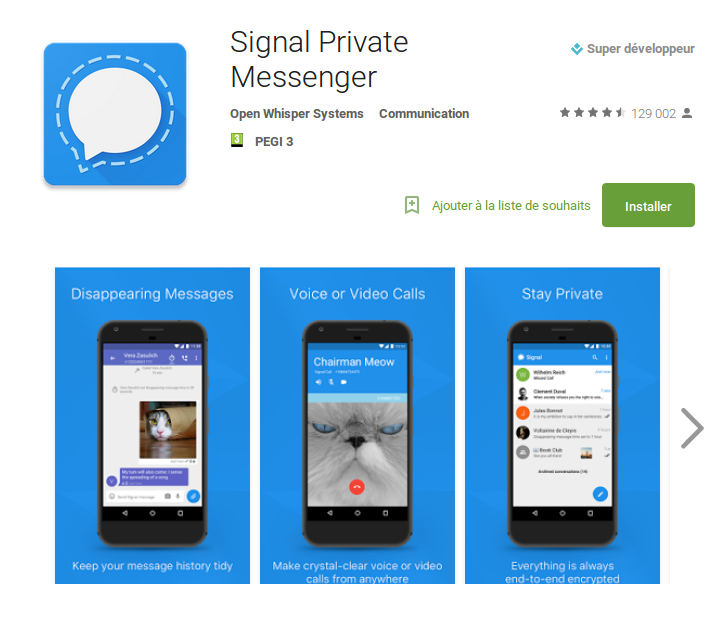
\includegraphics[scale=0.3] {./images/Signal_PlayStore.png} 
\end{center}


\end{frame}

%----------------------------------------------------------------------------------------
\begin{frame}
\frametitle{Silence}
\begin{center}
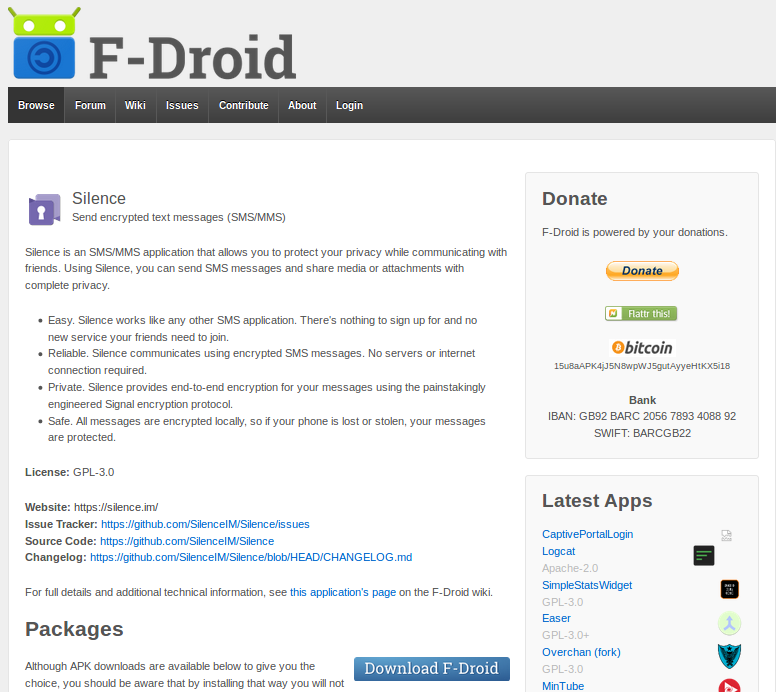
\includegraphics[scale=0.5] {./images/Silence_FDroid.png} 
\end{center}
\end{frame}

%----------------------------------------------------------------------------------------
\begin{frame}
\Huge{\centerline{Comment l'utiliser?}}
\end{frame}

%----------------------------------------------------------------------------------------
\begin{frame}
\frametitle{TODO}
\begin{block}{Liste des choses à présenter - Ajouter}
\begin{itemize}
\item Premier échange chiffré...
\item Valider le correspondant via sa clef...
\end{itemize}
\end{block}
\end{frame}

%----------------------------------------------------------------------------------------
\begin{frame}
\Huge{\centerline{Merci de votre attention.}}
\Huge{\centerline{Place aux questions.}}
\end{frame}

\end{document}
